
%\documentclass[a4paper, 12pt]{scrreprt}

\documentclass[a4paper, 12pt]{scrartcl}
%usepackage[german]{babel}

%\usepackage{amsmath}
%usepackage{color}
\usepackage[utf8]{inputenc}
\usepackage[T1]{fontenc}
\usepackage{wrapfig}
\usepackage{lipsum}% Dummy-Text

%%%%%%%%%%%%bis hierhin alle nötigen userpackage

\usepackage[utf8]{inputenc}
\usepackage{amsmath}
\usepackage{amsfonts}
\usepackage{amssymb}
\usepackage{graphicx}
%\usepackage{wrapfig}
\usepackage[ngerman]{babel}
\usepackage[left=25mm,top=25mm,right=25mm,bottom=25mm]{geometry}
%\usepackage{floatrow}
\setlength{\parindent}{0em}
\usepackage[font=footnotesize,labelfont=bf]{caption}
\numberwithin{figure}{section}
\numberwithin{table}{section}
\usepackage{subcaption}
\usepackage{float}
\usepackage{url}
\usepackage{fancyhdr}
\usepackage{array}
\usepackage{geometry}
%\usepackage[nottoc,numbib]{tocbibind}
\usepackage[pdfpagelabels=true]{hyperref}
\usepackage[font=footnotesize,labelfont=bf]{caption}
\usepackage[T1]{fontenc}
\usepackage {palatino}
%\usepackage[numbers,super]{natbib}
%\usepackage{textcomp}
\usepackage[version=4]{mhchem}
%\usepackage[utf8]{inputenc}
\usepackage[T1]{fontenc}
\usepackage[german]{babel}
\usepackage{amsmath} 
\usepackage{mathtools}
\usepackage{amssymb}
\usepackage{stmaryrd}
%\usepackage[spelling]

%\input{packageDavid.tex}



								%%% ab hier Formatierung des Grundgerüstest
								
%%%% Kopfzeile

%\input{Schriftart}



\begin{document}

%%\documentclass[a4paper, 12pt]{scrreprt}

\documentclass[a4paper, 12pt]{scrartcl}
%usepackage[german]{babel}

%\usepackage{amsmath}
%usepackage{color}
\usepackage[utf8]{inputenc}
\usepackage[T1]{fontenc}
\usepackage{wrapfig}
\usepackage{lipsum}% Dummy-Text

%%%%%%%%%%%%bis hierhin alle nötigen userpackage

\usepackage[utf8]{inputenc}
\usepackage{amsmath}
\usepackage{amsfonts}
\usepackage{amssymb}
\usepackage{graphicx}
%\usepackage{wrapfig}
\usepackage[ngerman]{babel}
\usepackage[left=25mm,top=25mm,right=25mm,bottom=25mm]{geometry}
%\usepackage{floatrow}
\setlength{\parindent}{0em}
\usepackage[font=footnotesize,labelfont=bf]{caption}
\numberwithin{figure}{section}
\numberwithin{table}{section}
\usepackage{subcaption}
\usepackage{float}
\usepackage{url}
\usepackage{fancyhdr}
\usepackage{array}
\usepackage{geometry}
%\usepackage[nottoc,numbib]{tocbibind}
\usepackage[pdfpagelabels=true]{hyperref}
\usepackage[font=footnotesize,labelfont=bf]{caption}
\usepackage[T1]{fontenc}
\usepackage {palatino}
%\usepackage[numbers,super]{natbib}
%\usepackage{textcomp}
\usepackage[version=4]{mhchem}


%\begin{document}
\thispagestyle{empty}

\begin{flushleft}
Robert Strothmann, 5040218\\ 
Jonas Schulz, 5153815\\ 
David Ueberle, 4903184\\ 
\end{flushleft}
\vspace*{0.3cm}
E-Mail 1, E-Mail 2, ueberleda@zedat.fu-berlin.de\\
\begin{center}
	\vspace*{1cm}
	\Large
	{ \bfseries Laborbericht / Versuchsprotokoll}\\
	\vspace*{1cm}
	{Versuchsnummer - Versuchstitel}\\
\end{center}
	\vspace*{1cm}
	{Datum der Versuchsdurchführung:}\\
	{Datum der Protokolleinreichung:}\\
	{Assistent/in:}\\
	{Dateiname:}	
	\vfill
\begin{flushleft}
Mit der Einreichung wird versichert, dass das Protokoll von den oben eingetragenen Personen in gemeinschaftlicher Arbeit angefertigt worden ist und dass sämtliche Quellen, die zur Erstellung des Protokolls genutzt wurden, im 8. Teil des Protokolls (Literatur) kenntlich gemacht worden sind.
\end{flushleft}

\normalsize
\newpage
%\end{document}

%\twocolumn
\documentclass[a4paper]{scrartcl}

\begin{document}

\section{Einleitung}

Vielen Eigenschaften von Molekülen liegt eine quantenmechanische Betrachtung zugrunde. Mit der Schrödingergleichung ist es möglich zum Beispiel Potentialenergieflächen zu berechnen, die einem Informationen zu den charakteristischen Schwingungen  geben. Jedoch steigt die Komplexität der Gleichung stark an, umso größer die Systeme werden. Eine Möglichkeit der Simplifizierung ist hier die Born-Oppenheimer-Näherung. Sie approximiert aufgrund der vielfach höheren Masse der Kerne im Vergleich zu den Elektronen, dass die Bewegungen der Kerne und die der Elektronen separierbar sind. Außerdem kann angenommen werden dass die kinetische Energie der Kerne gleich Null und somit die potentielle Energie konstant ist. Isotopeneffekte spielen aufgrund dieser Vereinfachung keine Rolle.
Durch Lösen der dieser Gleichungen kann nun das Potential bei unterschiedlichen Kern-Kern Abständen berechnet werden, wodurch man die Potentialenergieflächen erhält.
Für den Grundzusatnd und für die angeregten Zustände ergeben sich unterschiedliche Potentialenergieflächen und somit auch unterschiedliche Gleichgewichtsabstände. Im Folgenden wird nur der Grundzustand betrachtet.




\end{document}







%%\documentclass[a4paper, 12pt]{scrreprt}

\documentclass[a4paper, 12pt]{scrartcl}
%usepackage[german]{babel}

%\usepackage{amsmath}
%usepackage{color}
\usepackage[utf8]{inputenc}
\usepackage[T1]{fontenc}
\usepackage{wrapfig}
\usepackage{lipsum}% Dummy-Text

%%%%%%%%%%%%bis hierhin alle nötigen userpackage

\usepackage[utf8]{inputenc}
\usepackage{amsmath}
\usepackage{amsfonts}
\usepackage{amssymb}
\usepackage{graphicx}
%\usepackage{wrapfig}
\usepackage[ngerman]{babel}
\usepackage[left=25mm,top=25mm,right=25mm,bottom=25mm]{geometry}
%\usepackage{floatrow}
\setlength{\parindent}{0em}
\usepackage[font=footnotesize,labelfont=bf]{caption}
\numberwithin{figure}{section}
\numberwithin{table}{section}
\usepackage{subcaption}
\usepackage{float}
\usepackage{url}
\usepackage{fancyhdr}
\usepackage{array}
\usepackage{geometry}
%\usepackage[nottoc,numbib]{tocbibind}
\usepackage[pdfpagelabels=true]{hyperref}
\usepackage[font=footnotesize,labelfont=bf]{caption}
\usepackage[T1]{fontenc}
\usepackage {palatino}
%\usepackage[numbers,super]{natbib}
%\usepackage{textcomp}
\usepackage[version=4]{mhchem}
%\begin{document}

\section{Theoretische Grundlagen}
\subsection{Quantentheorie :}
Die im Folgenden beschriebenen Systeme werden über die zeitunabhängige Schrödingergleichung ausgrdückt (Eq. 1). 

\begin {equation}
\mathcal{H}\left(r,R\right)\Psi\left(r,R\right)=E\Psi\left(r,R\right)
\end {equation}
\\
Jedoch steigt die Komplexität der Gleichung stark an, umso größer die Systeme werden, da sämtliche Elektronen und Kerne betrachtet werden müssen. Eine Möglichkeit der Vereinfachung ist hier die Born-Oppenheimer-Näherung (Eq. 2). 

\begin {equation}
\mathcal{H}\left(r,R\right)=\mathcal{H}_{K}\left(R\right)+\mathcal{H}_{e}\left(r,R\right)
\end {equation}
\\
Der große Massenunterschied zwischen Atomkern und Elektronen lässt eine Separierung der Bewegungen dieser folgen. Ferner benutzt man eigentlich die deutlich geringeren Geschwindigkeit einer Kernbewegung im Bezug zur Elektronenbewegung, basierend auf den unterschiedlichen Massen. Diese Überlegung führt zur Schlussfolgerung, dass die kinetische Energie der Kerne bei konstantem Kernabstand keinen Einfluss auf die Elektronen besitzt, folglich nur ein parametrisches Potential der beteiligten Kernabstände resultiert. Es ergibt sich die elektronische Schrödingergleichung (Eq. 3) mit dem Hamilton-Operator wobei die Energie nur noch parametrisch von den Koordinaten der Kerne abhängig ist.

\begin {equation}
\mathcal{H}_e\left(r,R\right)\Psi\left(r,R\right)=\left(E\left(R\right)-\mathcal{V}_{KK}\left(R\right)\right)\Psi_e\left(r,R\right)
\end {equation}
\\
Die Potentialfläche bezogen auf die Gesamtenergie des Systems über dem Bindungsabstand folgt aus der Lösung der zuvor beschriebenen elektronischen Schrödingergleichung. Durch die Born-Oppenheimer-Näherung spielen Isotopeneffekte keine Rolle, da die Kerne als in Ruhe approximiert werden und somit keine kinetische Energie besitzen. Die einzigen Terme in denen die Masse der Kerne vorkommen entfallen somit. Die Potentialenergieflächen sind abhängig von dem elektronischen Zustand des Moleküls, da die Schrödingergleichung über die Wellenfunktion mit den Quantenzahlen verbunden ist. Für die Schwingungsspektroskopie ist der Grundzustand besonders relevant, da sich die meisten physikochemische Fragestellungen aufgrund von praxisnähe auf Systeme im Grundzustand beschränken. Der Grundzustand verdeutlich in der Regel einen hochpopulierten Gleichgewichtszustand. Ferner ist die Detektion von kurzlebigen, angeregten Zuständen (wenn überhaupt möglich) nicht trivial.
\subsection{Verwendete Methoden :}
Zur Bestimmung der gesuchten Energiewerte bezogen auf die Bindungslänge der zweiatomigen Moleküle CO und HCl wurde mithilfe des Programms -Gaussian- die zeitunabhängige Schrödingergleichung gelöst. Im Allgemeinen berechnet -Gaussian- die Wellenfunktion im Rahmen der Born-Oppenheimer-Näherung genau für eine Kerngeometrie. Folglich wurde ein Intervall von Bindungslängen der betreffenden Moleküle gewählt, und jeweils für jede Geometrie ein Energiewert bestimmt, um representative Ergebnisse zu erhalten.\\	
\\
Berechnet wurden die Energien für beide Moleküle mit selbem Intervall an Bindungslängen in zwei vorimplementierten Methoden (B3LYP \& CCSD). Allgemein bestehen die unterschiede der Methoden in den verwendeten Näherungen, um Elektron-Elektron WW zu beschreiben. Im wesentlichen beruhen die Näherung auf Dichtefunktionalen für Elektronen und der daraus resultierenden WW (DFT) oder auf Beschreibung wirkenden Kräfte auf den Elektronen durch ein externes Kraftfeld (HF). Generell gibt es Unterscheidungen von verwendeten quantenmechanischen Methoden, die sich auf die Wahl der Parameter (z.B empirisch) beziehen. Desweiteren gibt es auch die Unterscheidbarkeit basierend auf den mathematischen Weg, wie die betreffenden Funktionale für Elektron-Elektron WW konstruiert werden.  Relativistische Effekte der Elektronen können bei leichten Atomen im Molekül wie HCl und CO vernachlässigt werden. Sollte dies nicht der Fall sein, müssen diese explizit durch Korrelationseffekte berücksichtigt werden. Der bei allen Berechnungen verwendete Basissatz (6-31G/6-31*) aus modifizierten Wasserstofforbitalen wurde, aufgrund geringer Anzahl an Basen, was eine geringe Rechenzeit bewirkt, und auf die Komplexität der Basen bezogen gute Qualität, gewählt.\\


%\end{document}

%\documentclass[12pt, letterpaper]{article}

 
%\begin{document}
\section{Durchführung}
Die Prozessierung erfolgt durch einen input file, welcher alle wichtigen Informationen der durchzuführenden Berechnung dem Computer übergibt. Dieser file beinhaltet im wesentlichen drei wichtige Blöcke. Der erste Befehlsblock am Anfang bezieht sich auf zugewiesene hardware Rechte, der folgende Block übergibt die Methode sowie weitere frei wählbare, vorimplementierte Optionen für die Berechnung (z.B die rekursive Berechnung für mehrere vordefinierte Bindungsabstände). Der letzte Block beinhaltet im wesentlichen die Eigenschaften des betrachteten quantenmechanischen Systems, wie die Gesamtladung, Spineigenschaften, sowie Atomtypen und Geometrien. Die Geometrien können sowohl in kartesischen Koordinaten, als auch in einer Z-Matrix angegeben sein. Die Darstellung in der Z-Matrix impliziert eine besonders große Vergleichbarkeit von geometrischen Eigenschaften wie Bindungslängen/- Winkeln und Torsionswinkeln im Molekül zu weiteren Referenzsystemen mit gleichem betrachteten Molekül.\\
\\
Zur Analyse wurden die zu berechnenden Daten aus dem output file manuell exportiert und weiter in -python- bearbeitet.

%\end{document}

%%\documentclass[a4paper, 12pt]{scrreprt}

\documentclass[a4paper, 12pt]{scrartcl}
%usepackage[german]{babel}

%\usepackage{amsmath}
%usepackage{color}
\usepackage[utf8]{inputenc}
\usepackage[T1]{fontenc}
\usepackage{wrapfig}
\usepackage{lipsum}% Dummy-Text

%%%%%%%%%%%%bis hierhin alle nötigen userpackage

\usepackage[utf8]{inputenc}
\usepackage{amsmath}
\usepackage{amsfonts}
\usepackage{amssymb}
\usepackage{graphicx}
%\usepackage{wrapfig}
\usepackage[ngerman]{babel}
\usepackage[left=25mm,top=25mm,right=25mm,bottom=25mm]{geometry}
%\usepackage{floatrow}
\setlength{\parindent}{0em}
\usepackage[font=footnotesize,labelfont=bf]{caption}
\numberwithin{figure}{section}
\numberwithin{table}{section}
\usepackage{subcaption}
\usepackage{float}
\usepackage{url}
\usepackage{fancyhdr}
\usepackage{array}
\usepackage{geometry}
%\usepackage[nottoc,numbib]{tocbibind}
\usepackage[pdfpagelabels=true]{hyperref}
\usepackage[font=footnotesize,labelfont=bf]{caption}
\usepackage[T1]{fontenc}
\usepackage {palatino}
%\usepackage[numbers,super]{natbib}
%\usepackage{textcomp}
\usepackage[version=4]{mhchem}

%\begin{document}

\newcolumntype{L}[1]{>{\raggedright\arraybackslash}p{#1}} % linksbündig mit Breitenangabe
\newcolumntype{C}[1]{>{\centering\arraybackslash}p{#1}} % zentriert mit Breitenangabe
\newcolumntype{R}[1]{>{\raggedleft\arraybackslash}p{#1}} % rechtsbündig mit Breitenangabe

\section{Auswertung}


Die mittels Gaussian erhaltenen Gleichgewichtsabstände wurden in Tabelle~\ref{Tab.1} zusammengetragen. Dabei handelt es sich um den Atomabstand R, welcher bei den jeweiligen minimalsten Energiewerten einer Datenreihe zu finden ist. Die Dissoziationensenergie wurden erhalten, indem der größte Energiewert der Asymptote vom kleinsten Energiewert der Kurve subtrahiert worden ist.

 \begin{table}[H]
 \centering
 
 
 \caption{Berechnete Gleichgewichtsabstände und Dissoziationsenergien von HCl und CO aus den mittels GAUSSIAN erhaltenen Werten  mit der Methode B3LYP und dem Basissatz 6-31G bzw. der Methode CCSD und dem Basissatz 6-31G*. Ferner sind experimentell bestimmte Literaturwerte der zu untersuchenden Größen gezeigt.$^{[2]}$ $^{[3]}$}
 \begin{tabular}{L{0.1\textwidth}L{0.20\textwidth}C{0.3\textwidth}C{0.20\textwidth}C{0.20\textwidth}}
\multicolumn{2}{c}{}&\multicolumn{1}{c}{Gleichgewichtsabstand R}&\multicolumn{2}{c}{Dissoziationsenergie}\\
 
  Molekül  & Methode &  in Ängstrom &   in Hartree & in kJ/mol \\
  CO  &B3LYP & 1.17 &  0.48&1260 \\
  CO  & CCSD (SCF)&1.11 & 0.49&1290\\
  CO  & CCSD (MP2)&1.15 & 0.59&1550\\
  CO  & CCSD (MP3)&1.13 & 0.55&1440\\
    CO&Literatur&	1.128323&&1077\\

  HCl  &B3LYP& 1.33 &  0.19&498\\
  HCl  & CCSD (SCF)&1.27  & 0.34&892\\
  HCl  & CCSD (MP2)&1.28  & 0.19&498\\
  HCl  & CCSD (MP3)&1.28  & 0.16&420\\
  HCl&Literatur&	1.27455&&429\\

\\
   
   
 \end{tabular}
 \label{Tab.1}
 \end{table}




\begin{table}[htbp]
  \centering
   \caption{Berechnete Gleichgewichtsabstände und Dissoziationsenergien von HCl und CO aus den mittels GAUSSIAN erhaltenen Werten  mit der Methode B3LYP und dem Basissatz 6-31G bzw. der Methode CCSD und dem Basissatz 6-31G*.}
  \begin{tabularx}{\columnwidth}{XL{0.15\textwidth}L{0.20\textwidth}L{0.10\textwidth}L{0.10\textwidth}}
\multicolumn{2}{c}{}&\multicolumn{1}{c}{Gleichgewichtsabstand}&\multicolumn{2}{c}{Dissoziationsenergie}\\
    
      Molekül  & Methode &  R in Ängstrom &   in Hartree & in kJ/mol \\
      \toprule[2pt]
  CO  &B3LYP & 1.17 &  0.48&1260 \\
  CO  & CCSD (SCF)&1.11 & 0.49&1290\\
  CO  & CCSD (MP2)&1.15 & 0.59&1550\\
  CO  & CCSD (MP3)&1.13 & 0.55&1440\\
    CO&Literatur&	1.128323&&1077\\

  HCl  &B3LYP& 1.33 &  0.19&498.0\\
  HCl  & CCSD (SCF)&1.27  & 0.34&892\\
  HCl  & CCSD (MP2)&1.28  & 0.19&498\\
  HCl  & CCSD (MP3)&1.28  & 0.16&420\\
  HCl&Literatur&	1.27455&&429\\
    
  \end{tabularx}
\end{table}



\begin{figure}[ht]
	\centering	
	\begin{minipage}{0.5\textwidth}
	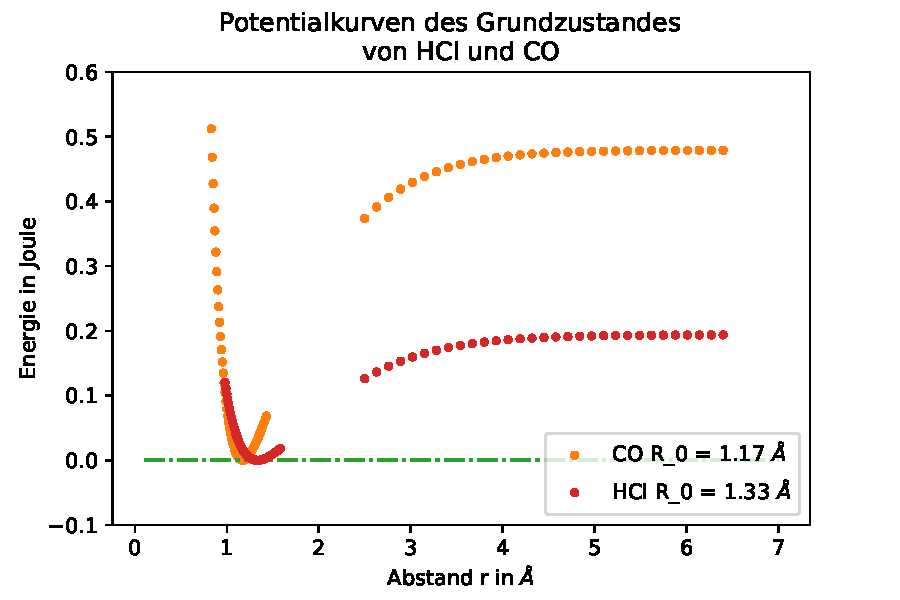
\includegraphics[width=\columnwidth]{Bilder/b3lypzusammen}
	\end{minipage}
	
	
	\caption{Grafische Auftragung der mit der Born-Oppenheimer-Näherung erhaltenen Energien bei verschiedenen Kernabständen von HCl und CO. Die Werte wurden mittels GAUSSIAN mit der Methode B3LYP und dem Basissatz 6-31G erhalten.}
	
	
	\label{b3lypzusammen}
\end{figure}


Wie in Abbildung~\ref{b3lypzusammen} zu sehen beschreiben die mit B3LYP errechneten Werte den Verlauf eines Morsepotentials. Es sei hier erwähnt, dass das tatsächliche Minimum der Kurven nicht bei Null liegt, sondern das Minimum von allen Energiewerten Subtrahiert worden ist, um dieses als Nullpunkt zu definieren. Dadurch ist es nun möglich anhand der Grafen eine qualitative Aussage über die Dissoziationsenergie, sowie den Gleichgewichtsabstand zu machen.


  

 
\begin{figure}[H]
	
\begin{minipage}{0.5\textwidth}
	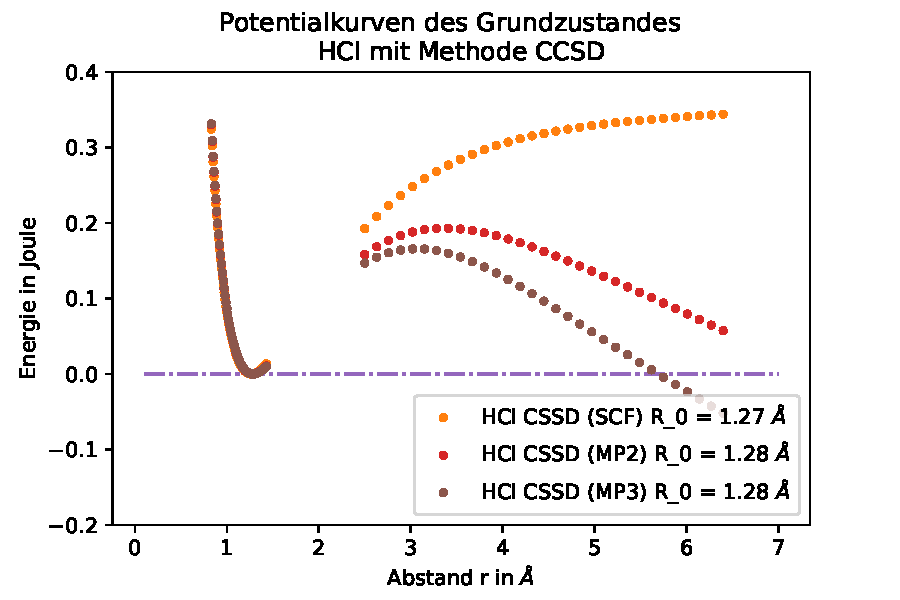
\includegraphics[width=\textwidth]{Bilder/HCl_CCSD}
\end{minipage}
\begin{minipage}{0.5\textwidth}
	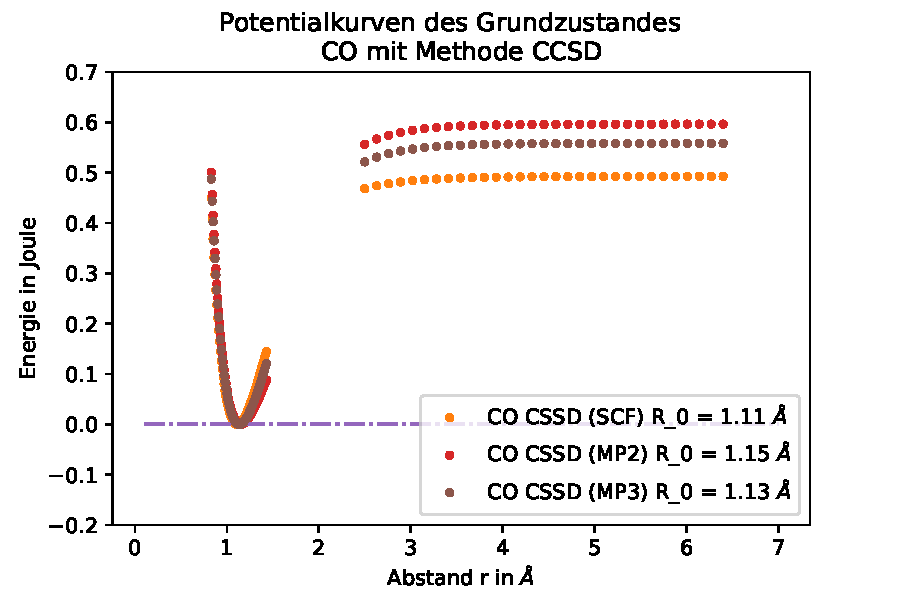
\includegraphics[width=\textwidth]{Bilder/CO_CCSD}
\end{minipage}


<<<<<<< HEAD
\caption{Grafische Auftragung der mit der Born-Oppenheimer-Näherung erhaltenen Energien bei verschiedenen Kernabständen von HCl und CO. Die Werte wurden mittels GAUSSIAN mit der Methode CCSD und dem Basissatz 6-31G* erhalten.}
=======
\caption{Grafische Auftragung der mit der Born-Oppenheimer-Näherung erhaltenen Energien bei verschiedenen Kernabständen von HCl und CO. Die Werte wurden mittels GAUSSIAN mit der Methode CCSD und dem Basissatz 6-31G* erhalten. Die Grafiken wurde mit Python erstellt und über Spyder ausgegeben.}
>>>>>>> 8fd6c09d67ca1bf8d526d13bea9bbc5b6adec26b


	\label{HCl_CCSD}
\end{figure}


Der Verlauf der Werte, welche durch die CCSD Methode für CO, sowie HCl erhalten wurden, sind in Abbildung~\ref{HCl_CCSD} aufgetragen worden. Bei der Betrachtung der Werte kann beobachtet werden, dass die Entwicklung durch CCSD um das Minimum noch etwas genauer, als es mittels B3LYP der Fall war, gelungen ist. Jedoch beschreibt die Energie  nach der Dissoziation des Moleküle besonders bei HCl einen Verlauf der gänzlich den Erwartungen widerspricht. Die Kurven sollten eigentlich gegen einen Energiewert konvergieren. 


\section{Zusammenfassung}

Die erhaltenen Bindungslängen stimmen in guter Näherung mit den Literaturwerten überein (siehe Tabelle~\ref{Tab.1}.) 
Die mittels der CCSD-Methode gewonnenen Werte nähern sich besser an den Gleichgewichtsabstand der Literatur an als die mit der B3LYP Methode. Die ermittelten Dissoziationsenergien für das CO Molekül sind wie zu erwarten wesentlich größer gegenüber dem HCl Molekül. Die Werte decken sich jedoch deutlich schlechter mit der Literatur als es bei dem Gleichgewichtsabstand der Fall ist. Im Allgemeinen sind jedoch richtige Größenordnung und richtige Relation zu erkennen.



 
 






%\end{document}

\newpage
%%\documentclass[a4paper, 12pt]{scrreprt}

\documentclass[a4paper, 12pt]{scrartcl}
%usepackage[german]{babel}

%\usepackage{amsmath}
%usepackage{color}
\usepackage[utf8]{inputenc}
\usepackage[T1]{fontenc}
\usepackage{wrapfig}
\usepackage{lipsum}% Dummy-Text

%%%%%%%%%%%%bis hierhin alle nötigen userpackage

\usepackage[utf8]{inputenc}
\usepackage{amsmath}
\usepackage{amsfonts}
\usepackage{amssymb}
\usepackage{graphicx}
%\usepackage{wrapfig}
\usepackage[ngerman]{babel}
\usepackage[left=25mm,top=25mm,right=25mm,bottom=25mm]{geometry}
%\usepackage{floatrow}
\setlength{\parindent}{0em}
\usepackage[font=footnotesize,labelfont=bf]{caption}
\numberwithin{figure}{section}
\numberwithin{table}{section}
\usepackage{subcaption}
\usepackage{float}
\usepackage{url}
\usepackage{fancyhdr}
\usepackage{array}
\usepackage{geometry}
%\usepackage[nottoc,numbib]{tocbibind}
\usepackage[pdfpagelabels=true]{hyperref}
\usepackage[font=footnotesize,labelfont=bf]{caption}
\usepackage[T1]{fontenc}
\usepackage {palatino}
%\usepackage[numbers,super]{natbib}
%\usepackage{textcomp}
\usepackage[version=4]{mhchem}
%\begin{document}

\section{Literaturverzeichnis}
1. W. Kutzelnigg, Einführung in die Theoretische Chemie, Wiley-VCH, Weinheim 2001
\\
\\
2. NIST Webbook - link : https://webbook.nist.gov
\\
\\
3. A. F. Holleman \& Nils Wiberg, Lehrbuch der anorganischen Chemie,  de Gruyter, New York 2016
%\end{document}


%\input{Ergänzendefragen}
\newpage
\section{Rohdaten}
 
 \begin{longtable}{{L{0.25\textwidth}L{0.25\textwidth}L{0.25\textwidth}L{0.25\textwidth}}}

\caption{Rohdaten der Energien nach Born Oppenheimer Näherung für verschiedene Bindungsabstände berechnet über GAUSSIAN für HCl und CO mit der Methode B3LYP und dem Basissatz 6-31G}\\
\multicolumn{2}{c}{B3LYP Werte für HCL}&\multicolumn{2}{c}{B3LYP Werte für CO}\\
Atomabstand in Ängstrom&Energie in Hatree&Atomabstand in Ängstrom&Energie in Hartree\\
\endfirsthead
\multicolumn{2}{c}{B3LYP Werte für HCL}&\multicolumn{2}{c}{B3LYP Werte für CO}\\
Atomabstand in Ängstrom&Energie in Hatree&Atomabstand in Ängstrom&Energie in Hartree\\
\endhead
0.83&-112.7369&0.98&-460.63329\\
0.84&-112.78074&0.99&-460.64262\\
0.85&-112.82153&1.0&-460.65139\\
0.86&-112.85945&1.01&-460.65961\\
0.87&-112.89468&1.02&-460.66733\\
0.88&-112.92737&1.03&-460.67456\\
0.89&-112.95769&1.04&-460.68134\\
0.9&-112.98577&1.05&-460.68768\\
0.91&-113.01175&1.06&-460.6936\\
0.92&-113.03576&1.07&-460.69913\\
0.93&-113.05792&1.08&-460.70429\\
0.94&-113.07834&1.09&-460.70909\\
0.95&-113.09713&1.1&-460.71356\\
0.96&-113.11438&1.11&-460.7177\\
0.97&-113.1302&1.12&-460.72154\\
0.98&-113.14466&1.13&-460.72509\\
0.99&-113.15786&1.14&-460.72836\\
1.0&-113.16986&1.15&-460.73137\\
1.01&-113.18075&1.16&-460.73414\\
1.02&-113.1906&1.17&-460.73667\\
1.03&-113.19946&1.18&-460.73898\\
1.04&-113.2074&1.19&-460.74109\\
1.05&-113.21448&1.2&-460.74299\\
1.06&-113.22075&1.21&-460.7447\\
1.07&-113.22626&1.22&-460.74623\\
1.08&-113.23107&1.23&-460.74759\\
1.09&-113.23521&1.24&-460.74878\\
1.1&-113.23873&1.25&-460.74983\\
1.11&-113.24167&1.26&-460.75072\\
1.12&-113.24406&1.27&-460.75148\\
1.13&-113.24595&1.28&-460.75211\\
1.14&-113.24737&1.29&-460.75262\\
1.15&-113.24835&1.3&-460.75301\\
1.16&-113.24891&1.31&-460.75329\\
1.17&-113.2491&1.32&-460.75347\\
1.18&-113.24892&1.33&-460.75355\\
1.19&-113.24841&1.34&-460.75353\\
1.2&-113.24759&1.35&-460.75343\\
1.21&-113.24649&1.36&-460.75324\\
1.22&-113.24512&1.37&-460.75298\\
1.23&-113.2435&1.38&-460.75263\\
1.24&-113.24165&1.39&-460.75222\\
1.25&-113.23959&1.4&-460.75174\\
1.26&-113.23734&1.41&-460.7512\\
1.27&-113.2349&1.42&-460.7506\\
1.28&-113.2323&1.43&-460.74995\\
1.29&-113.22955&1.44&-460.74924\\
1.3&-113.22666&1.45&-460.74849\\
1.31&-113.22363&1.46&-460.74769\\
1.32&-113.2205&1.47&-460.74685\\
1.33&-113.21725&1.48&-460.74596\\
1.34&-113.21391&1.49&-460.74504\\
1.35&-113.21048&1.5&-460.74409\\
1.36&-113.20696&1.51&-460.74309\\
1.37&-113.20338&1.52&-460.74207\\
1.38&-113.19974&1.53&-460.74101\\
1.39&-113.19603&1.54&-460.73993\\
1.4&-113.19228&1.55&-460.73883\\
1.41&-113.18848&1.56&-460.73769\\
1.42&-113.18465&1.57&-460.73654\\
1.43&-113.18078&1.58&-460.73537\\
2.5&-112.87545&2.5&-460.62736\\
2.63&-112.85758&2.63&-460.61709\\
2.76&-112.84261&2.76&-460.60812\\
2.89&-112.83006&2.89&-460.6004\\
3.02&-112.81951&3.02&-460.59381\\
3.15&-112.81066&3.15&-460.5882\\
3.28&-112.80324&3.28&-460.58345\\
3.41&-112.79705&3.41&-460.57944\\
3.54&-112.79191&3.54&-460.57606\\
3.67&-112.78767&3.67&-460.57323\\
3.8&-112.78418&3.8&-460.57086\\
3.93&-112.78133&3.93&-460.56888\\
4.06&-112.77902&4.06&-460.56724\\
4.19&-112.77715&4.19&-460.56587\\
4.32&-112.77565&4.32&-460.56474\\
4.45&-112.77446&4.45&-460.56381\\
4.58&-112.77352&4.58&-460.56304\\
4.71&-112.77279&4.71&-460.5624\\
4.84&-112.77221&4.84&-460.56189\\
4.97&-112.77177&4.97&-460.56146\\
5.1&-112.77143&5.1&-460.56112\\
5.23&-112.77116&5.23&-460.56083\\
5.36&-112.77095&5.36&-460.5606\\
5.49&-112.77079&5.49&-460.56042\\
5.62&-112.77066&5.62&-460.56028\\
5.75&-112.77055&5.75&-460.56016\\
5.88&-112.77046&5.88&-460.56006\\
6.01&-112.77039&6.01&-460.55998\\
6.14&-112.77032&6.14&-460.55991\\
6.27&-112.77026&6.27&-460.55986\\
6.4&-112.7702&6.4&-460.55982\\

  

 \label{Tab.rohdatenb3lyp}
 \end{longtable}
 
 
  \begin{longtable}{{L{0.25\textwidth}L{0.25\textwidth}L{0.25\textwidth}L{0.25\textwidth}}}
\caption{Rohdaten der Energien nach Born Oppenheimer Näherung für verschiedene Bindungsabstände berechnet über GAUSSIAN für HCl mit der Methode CCSD und dem Basissatz 6-31G*}\\  
  &\multicolumn{3}{c}{Enegien nach der CCSD Methode für HCl}\\
Atomabstand in Ängstrom&(SCF) in Hartree&(MP2) in Hartree&(MP3) in Hartree\\
\endfirsthead

&\multicolumn{3}{c}{Enegien nach der CCSD Methode für HCl}\\
Atomabstand in Ängstrom&(SCF) in Hartree&(MP2) in Hartree&(MP3) in Hartree\\
\endhead

0.83&-112.28837&-112.52057&-112.53124\\
0.84&-112.33083&-112.56469&-112.57517\\
0.85&-112.37019&-112.60571&-112.61597\\
0.86&-112.40663&-112.6438&-112.65385\\
0.87&-112.44032&-112.67915&-112.68897\\
0.88&-112.47143&-112.71192&-112.72149\\
0.89&-112.50012&-112.74226&-112.75157\\
0.9&-112.52652&-112.77031&-112.77936\\
0.91&-112.55077&-112.79622&-112.80499\\
0.92&-112.57301&-112.82012&-112.82858\\
0.93&-112.59334&-112.84211&-112.85027\\
0.94&-112.6119&-112.86233&-112.87016\\
0.95&-112.62878&-112.88087&-112.88836\\
0.96&-112.64408&-112.89784&-112.90497\\
0.97&-112.6579&-112.91334&-112.92009\\
0.98&-112.67033&-112.92744&-112.9338\\
0.99&-112.68145&-112.94025&-112.9462\\
1.0&-112.69135&-112.95183&-112.95735\\
1.01&-112.7001&-112.96226&-112.96734\\
1.02&-112.70776&-112.97162&-112.97624\\
1.03&-112.71441&-112.97997&-112.98411\\
1.04&-112.7201&-112.98738&-112.99101\\
1.05&-112.7249&-112.9939&-112.99701\\
1.06&-112.72887&-112.99959&-113.00216\\
1.07&-112.73204&-113.0045&-113.00651\\
1.08&-112.73448&-113.00868&-113.01011\\
1.09&-112.73623&-113.01219&-113.01301\\
1.1&-112.73734&-113.01505&-113.01524\\
1.11&-112.73784&-113.01732&-113.01686\\
1.12&-112.73777&-113.01904&-113.0179\\
1.13&-112.73718&-113.02024&-113.0184\\
1.14&-112.73609&-113.02095&-113.01839\\
1.15&-112.73454&-113.02121&-113.01791\\
1.16&-112.73256&-113.02106&-113.01697\\
1.17&-112.73018&-113.02051&-113.01563\\
1.18&-112.72742&-113.0196&-113.01389\\
1.19&-112.72432&-113.01835&-113.01179\\
1.2&-112.7209&-113.01679&-113.00935\\
1.21&-112.71717&-113.01494&-113.00659\\
1.22&-112.71317&-113.01282&-113.00354\\
1.23&-112.70891&-113.01046&-113.00021\\
1.24&-112.70441&-113.00786&-112.99662\\
1.25&-112.69969&-113.00506&-112.99279\\
1.26&-112.69477&-113.00206&-112.98874\\
1.27&-112.68966&-112.99888&-112.98449\\
1.28&-112.68439&-112.99554&-112.98004\\
1.29&-112.67895&-112.99205&-112.97541\\
1.3&-112.67338&-112.98843&-112.97061\\
1.31&-112.66767&-112.98467&-112.96567\\
1.32&-112.66185&-112.98081&-112.96058\\
1.33&-112.65593&-112.97684&-112.95535\\
1.34&-112.6499&-112.97278&-112.95001\\
1.35&-112.6438&-112.96863&-112.94456\\
1.36&-112.63762&-112.96441&-112.939\\
1.37&-112.63137&-112.96011&-112.93335\\
1.38&-112.62507&-112.95576&-112.92761\\
1.39&-112.61872&-112.95134&-112.9218\\
1.4&-112.61233&-112.94688&-112.91591\\
1.41&-112.6059&-112.94237&-112.90996\\
1.42&-112.59945&-112.93781&-112.90395\\
1.43&-112.59298&-112.93322&-112.89788\\
2.5&-112.26977&-112.46478&-112.49705\\
2.63&-112.26398&-112.45445&-112.48758\\
2.76&-112.25963&-112.44681&-112.48062\\
2.89&-112.25634&-112.44115&-112.47546\\
3.02&-112.25383&-112.43695&-112.47163\\
3.15&-112.25192&-112.43385&-112.46877\\
3.28&-112.25044&-112.43155&-112.46664\\
3.41&-112.24931&-112.42985&-112.46505\\
3.54&-112.24842&-112.42859&-112.46386\\
3.67&-112.24774&-112.42766&-112.46296\\
3.8&-112.2472&-112.42696&-112.46229\\
3.93&-112.24679&-112.42645&-112.46179\\
4.06&-112.24647&-112.42606&-112.46142\\
4.19&-112.24622&-112.42577&-112.46114\\
4.32&-112.24603&-112.42556&-112.46093\\
4.45&-112.24589&-112.4254&-112.46078\\
4.58&-112.24577&-112.42528&-112.46066\\
4.71&-112.24568&-112.42518&-112.46056\\
4.84&-112.24561&-112.42511&-112.46049\\
4.97&-112.24555&-112.42505&-112.46043\\
5.1&-112.2455&-112.425&-112.46038\\
5.23&-112.24546&-112.42495&-112.46034\\
5.36&-112.24543&-112.42492&-112.4603\\
5.49&-112.2454&-112.42489&-112.46027\\
5.62&-112.24537&-112.42486&-112.46025\\
5.75&-112.24535&-112.42484&-112.46023\\
5.88&-112.24533&-112.42482&-112.46021\\
6.01&-112.24531&-112.4248&-112.46019\\
6.14&-112.2453&-112.42479&-112.46017\\
6.27&-112.24528&-112.42477&-112.46016\\
6.4&-112.24527&-112.42476&-112.46015\\
 \label{Tab.rohdatenCCSDHCl}
 \end{longtable}

  \begin{longtable}{{L{0.25\textwidth}L{0.25\textwidth}L{0.25\textwidth}L{0.25\textwidth}}}
  \caption{Rohdaten der Energien nach Born Oppenheimer Näherung für verschiedene Bindungsabstände berechnet über GAUSSIAN für HCl mit der Methode CCSD und dem Basissatz 6-31G*}\\
  
&\multicolumn{3}{c}{Energien nach der CCSD Methode für CO}\\
Atomabstand in Ängstrom&(SCF) in Hartree&(MP2) in Hartree&(MP3) in Hartree\\

\endfirsthead 

&\multicolumn{3}{c}{Energien nach der CCSD Methode für CO}\\
Atomabstand in Ängstrom&(SCF) in Hartree&(MP2) in Hartree&(MP3) in Hartree\\
\endhead

0.83&-459.73567&-459.86221&-459.87618\\
0.84&-459.75776&-459.88436&-459.89835\\
0.85&-459.77861&-459.90528&-459.91929\\
0.86&-459.79828&-459.92503&-459.93906\\
0.87&-459.81684&-459.94366&-459.95771\\
0.88&-459.83434&-459.96124&-459.9753\\
0.89&-459.85082&-459.97781&-459.9919\\
0.9&-459.86635&-459.99342&-460.00753\\
0.91&-459.88097&-460.00813&-460.02226\\
0.92&-459.89472&-460.02197&-460.03613\\
0.93&-459.90764&-460.035&-460.04918\\
0.94&-459.91979&-460.04724&-460.06145\\
0.95&-459.93119&-460.05875&-460.07298\\
0.96&-459.94188&-460.06955&-460.08381\\
0.97&-459.9519&-460.07969&-460.09396\\
0.98&-459.96128&-460.08919&-460.10349\\
0.99&-459.97006&-460.09808&-460.11241\\
1.0&-459.97826&-460.1064&-460.12076\\
1.01&-459.98591&-460.11418&-460.12856\\
1.02&-459.99304&-460.12144&-460.13585\\
1.03&-459.99968&-460.12821&-460.14264\\
1.04&-460.00585&-460.13451&-460.14897\\
1.05&-460.01157&-460.14036&-460.15486\\
1.06&-460.01686&-460.1458&-460.16032\\
1.07&-460.02175&-460.15083&-460.16538\\
1.08&-460.02626&-460.15548&-460.17006\\
1.09&-460.03041&-460.15977&-460.17438\\
1.1&-460.0342&-460.16372&-460.17836\\
1.11&-460.03768&-460.16734&-460.18201\\
1.12&-460.04083&-460.17065&-460.18535\\
1.13&-460.0437&-460.17367&-460.1884\\
1.14&-460.04628&-460.17641&-460.19117\\
1.15&-460.0486&-460.17889&-460.19368\\
1.16&-460.05066&-460.18111&-460.19593\\
1.17&-460.05248&-460.1831&-460.19795\\
1.18&-460.05408&-460.18486&-460.19974\\
1.19&-460.05545&-460.1864&-460.20132\\
1.2&-460.05663&-460.18774&-460.20269\\
1.21&-460.05761&-460.18889&-460.20387\\
1.22&-460.05841&-460.18986&-460.20487\\
1.23&-460.05903&-460.19066&-460.2057\\
1.24&-460.05949&-460.19129&-460.20637\\
1.25&-460.05979&-460.19177&-460.20688\\
1.26&-460.05995&-460.1921&-460.20725\\
1.27&-460.05997&-460.19229&-460.20747\\
1.28&-460.05985&-460.19236&-460.20757\\
1.29&-460.05961&-460.1923&-460.20755\\
1.3&-460.05926&-460.19212&-460.20741\\
1.31&-460.05879&-460.19184&-460.20716\\
1.32&-460.05822&-460.19145&-460.20681\\
1.33&-460.05755&-460.19096&-460.20636\\
1.34&-460.05679&-460.19038&-460.20582\\
1.35&-460.05594&-460.18972&-460.20519\\
1.36&-460.05501&-460.18897&-460.20449\\
1.37&-460.054&-460.18815&-460.2037\\
1.38&-460.05292&-460.18726&-460.20285\\
1.39&-460.05177&-460.1863&-460.20193\\
1.4&-460.05056&-460.18528&-460.20095\\
1.41&-460.04929&-460.1842&-460.19992\\
1.42&-460.04796&-460.18307&-460.19882\\
1.43&-460.04658&-460.18188&-460.19768\\
2.5&-459.86738&-460.0342&-460.06076\\
2.63&-459.85138&-460.02393&-460.05283\\
2.76&-459.83685&-460.01559&-460.04709\\
2.89&-459.82373&-460.0091&-460.04347\\
3.02&-459.81191&-460.00435&-460.04186\\
3.15&-459.80129&-460.00122&-460.04212\\
3.28&-459.79178&-459.99959&-460.04411\\
3.41&-459.78327&-459.99933&-460.04765\\
3.54&-459.77567&-460.00029&-460.05257\\
3.67&-459.7689&-460.00233&-460.05868\\
3.8&-459.76287&-460.00531&-460.0658\\
3.93&-459.7575&-460.00909&-460.07376\\
4.06&-459.75273&-460.01357&-460.0824\\
4.19&-459.74848&-460.01861&-460.09157\\
4.32&-459.7447&-460.02412&-460.10114\\
4.45&-459.74133&-460.03&-460.111\\
4.58&-459.73832&-460.0362&-460.12106\\
4.71&-459.73563&-460.04264&-460.13124\\
4.84&-459.7332&-460.04927&-460.14147\\
4.97&-459.73102&-460.05604&-460.15172\\
5.1&-459.72904&-460.06294&-460.16193\\
5.23&-459.72723&-460.06993&-460.17209\\
5.36&-459.72558&-460.07698&-460.18217\\
5.49&-459.72407&-460.0841&-460.19216\\
5.62&-459.72267&-460.09126&-460.20206\\
5.75&-459.72136&-460.09846&-460.21186\\
5.88&-459.72015&-460.10569&-460.22157\\
6.01&-459.71901&-460.11296&-460.23118\\
6.14&-459.71793&-460.12025&-460.24071\\
6.27&-459.71692&-460.12758&-460.25015\\
6.4&-459.71595&-460.13493&-460.25951\\

  
 
 \label{Tab.rohdatenCCSDCO}
 \end{longtable}

%\input{Zusammenfassung}

%%%\documentclass[a4paper, 12pt]{scrreprt}

\documentclass[a4paper, 12pt]{scrartcl}
%usepackage[german]{babel}

%\usepackage{amsmath}
%usepackage{color}
\usepackage[utf8]{inputenc}
\usepackage[T1]{fontenc}
\usepackage{wrapfig}
\usepackage{lipsum}% Dummy-Text

%%%%%%%%%%%%bis hierhin alle nötigen userpackage

\usepackage[utf8]{inputenc}
\usepackage{amsmath}
\usepackage{amsfonts}
\usepackage{amssymb}
\usepackage{graphicx}
%\usepackage{wrapfig}
\usepackage[ngerman]{babel}
\usepackage[left=25mm,top=25mm,right=25mm,bottom=25mm]{geometry}
%\usepackage{floatrow}
\setlength{\parindent}{0em}
\usepackage[font=footnotesize,labelfont=bf]{caption}
\numberwithin{figure}{section}
\numberwithin{table}{section}
\usepackage{subcaption}
\usepackage{float}
\usepackage{url}
\usepackage{fancyhdr}
\usepackage{array}
\usepackage{geometry}
%\usepackage[nottoc,numbib]{tocbibind}
\usepackage[pdfpagelabels=true]{hyperref}
\usepackage[font=footnotesize,labelfont=bf]{caption}
\usepackage[T1]{fontenc}
\usepackage {palatino}
%\usepackage[numbers,super]{natbib}
%\usepackage{textcomp}
\usepackage[version=4]{mhchem}
%\begin{document}

\section{Literaturverzeichnis}
1. W. Kutzelnigg, Einführung in die Theoretische Chemie, Wiley-VCH, Weinheim 2001
\\
\\
2. NIST Webbook - link : https://webbook.nist.gov
\\
\\
3. A. F. Holleman \& Nils Wiberg, Lehrbuch der anorganischen Chemie,  de Gruyter, New York 2016
%\end{document}



%\input{Rohdaten}

\end{document}